%%%%%%%%%%%%%%%%%%%%%%%%%%%%%%
\section{真实数据样本和MC样本}
本论文中,直接采用Trubo Stream真实数据用于分析,也就是说读出来的数据中$\psitwos \rightarrow\mu^{+}\mu^{-}$这一衰变道已经经过了重建。
在线选择我们采用了 {\it L0DiMuon }, {\it Hlt1DiMuonHighMass}和 {\it Hlt2DiMuonPsi2STurbo}三个触发选择条件,
具体条件如表~\ref{tab:trgSummary}所示。
\begin{table}[!ht]
\begin{center}
\caption {零级触发和高级触发的具体条件汇总表。}
\begin{tabular}{l|l}
\hline
触发条件&主要的选择条件\\
\hline
{\it L0DiMuon } &$p_{\rm T1}$ $\times$ $p_{\rm T2} >1.69(\gevc)^2$, nSPDHits$<900$\\
\hline
 \multirow{7}{*}{\it Hlt1DiMuonHighMass}												 & $p >6\gevc$\\
                         & $\pt >0.3\gevc$\\
                         & vertex DOCA  $<0.2$\\
                         & Track $\chisqndf<3$\\
												 & vertex $\chisqndf<25$ \\
												 & Muon ID: isMuon \\
                         & $m_{\mumu}>2.7\gevcc$\\
\hline
\multirow{2}{*}{\it Hlt2DiMuonPsi2STurbo}   & $|m_{\mumu}-m_{\psitwos}|<120\mevcc$\\
                                        & $\pt_{\psitwos}>2000\mevc$ \\
\hline
\end{tabular}
\label{tab:trgSummary} 
\end{center}
\end{table}

本论文利用$\lhcb$实验上2015年收集的$275\invpb$数据,采用了TCK0x10600A2, TCK0x10600A3, TCK0x10800A2和TCK0x11400A8触发条件选择之后的数据。
这几个选择条件针对$\mu$ 子的选择是一样的。它们对应的各自积分亮度如下所示:
\begin{itemize} 
\item $83.57\invpb$ with TCK 0x10600A2 MagDown;
\item $60.00\invpb$ with TCK 0x10600A3 MagDown;
\item $11.05\invpb$ with TCK 0x10800A2 MagDown;
\item $48.56\invpb$ with TCK 0x10800A2 MagUp;
\item $71.52\invpb$ with TCK 0x11400A8 MagUp.
\end{itemize}

$\lhcb$上针对效率的研究,采用的是蒙特卡洛(MC)样本,MC样本需要通过专门申请产生。
为研究接受度和重建效率,本论文产生了8M产生子水平的MC样本和8M全模拟型MC 样本。
简单介绍一下$\lhcb$上MC样本的模拟模块:PYTHIA软件产生$\pp$ 对撞数据,EVTGEN~\cite{Belyaev:2011zza}软件描述强子的衰变,用PHOTOS产生末态辐射,用GEANT4包描述粒子的产生及其相互作用。特别指出整个过程中,粲夸克偶素的模拟是非极化的。

\section{离线选择}

上文表~\ref{tab:trgSummary}已经表明,针对在线选择,本文采用了L0Dimuon、Hlt1Dimuon\\HighMass和Hlt2DimuonPsi2STurbo三个触发选择条件。为进一步提高信噪比,本文还进行了离线选择:在径迹的选择中,为了减少鬼径迹的影响,选择条件要求径迹是鬼径迹的概率小于0.3;
为了选择好的$\mu$ 径迹,要求径迹的重建质量$\chi^{2}/ndof$ 小于3, 每条径迹的横动量$\pt$大于1200MeV/c,赝快度$\eta$满足$2.0<\eta<4.9$), 并且对径迹做了粒子鉴别,要求被鉴别为$\mu$,具体的粒子鉴别要求IsMuon\&\& MC15TuneV1\_ProbNNmu*(1-MC15TuneV1\_ProbNNpi)> 0.6;
为了选择好的$\psitwos$的径迹,要求顶点$\chi^{2}$的$p$值大于0.5\%;
$\psitwos$的质量窗卡在了[3566,3806]$\mevcc$。
最终离线选择条件总结如表~\ref{tab:selections} 所示。

\begin{table}[!htb]
\tabcolsep 5mm
\begin{center}
\caption{$\psitwos \to \mu^+\mu^-$ 离线选择条件。}
\begin{tabular}{l|l}
\hline 变量& 选择条件 \\
\hline
径迹:鬼径迹概率 & $<0.3$\\
$\mu$: 横动量$\pt$ & $>1200\mevc$\\
$\mu$: 赝快度$\eta$ & $2.0<\eta<4.9$\\
$\mu$: 径迹质量 $ \chisqndf$&$<3$\\
$\mu$: 粒子鉴别 & \footnotesize {IsMuon \&\& MC15TuneV1\_ProbNNmu*(1-MC15TuneV1\_ProbNNpi) $>$ 0.6} \\
$\psitwos$: 顶点 $\mathrm{Prob}(\chisqndf)$ & $>0.5\%$\\
赝寿命 $t_{z}$ & $(-10, 10)\ps$\\
$t_{z}$的不确定性:& $<0.3ps$\\
$\psitwos$: 质量窗 &[3566, 3806]$\mevcc$ \\
$\psitwos$: 信号的零级触发 &  L0DiMuon\\
$\psitwos$: 信号的高级触发HLT1 &  Hlt1DiMuonHighMass\\
\hline
\end{tabular}
\label{tab:selections}
\end{center}
\end{table}

$\psitwos$的两种来源:$\pp$对撞直接产生和$b$强子飞行一段时间衰变产生,信号衰变链如~\ref{decay}所示:
\begin{figure}[!h]
\centering
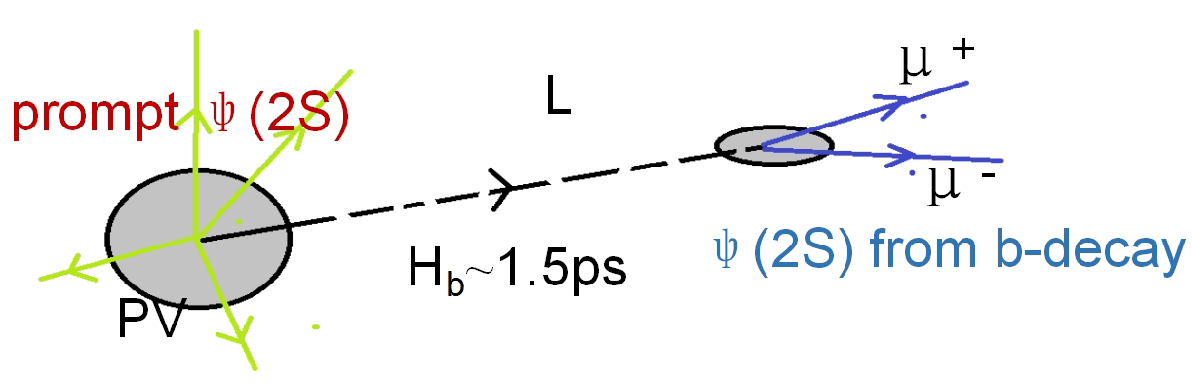
\includegraphics[width=0.8\textwidth]{chap3_detached}
\caption{两种信号$\psitwos$衰变链示意图。}
\label{decay}
\end{figure}
为提取$\pp$对撞直接产生的$\psitwos$介子和来自$b$衰变产生的$\psitwos$介子的信号数目,本文采用了变量赝寿命$t_{z}$,公式如下:

\begin{equation}\label{eq:tz}
t_z = \frac{(z_{\psitwos}-z_{\rm PV}) \times M_{\psitwos}}{p_z} \,,
\end{equation}

其中,$z_{\psitwos}$为$\psitwos$衰变顶点沿Z轴的分量;$z_{\rm pv}$为初始的$\pp$ 对撞顶点沿Z轴的分量;$M_{\psitwos}$为$\psitwos$的PDG质量;$p_{z}$为动量在z 轴上的投影。


\section{$\psitwos$微分产生截面测量}
本论文核心是测量$\psitwos$的微分产生截面,微分产生截面的测量公式有如下定义:
\begin{equation}
  \frac{\deriv^2\sigma}{\deriv y\deriv \pt} 
  = \frac{N(\psimumu)}
         {\lum\times\etot\times \BR(\psimumu)\times\Delta y \times \Delta \pt}. 
\label{eq:CrossSec}
\end{equation}

其中:
\begin{itemize}
\item $N(\psitwos\rightarrow\mu^{+}\mu^{-})$是给定($\pt$,$y$)内拟合得到的信号数目;
\item $\mathcal L$ 是总的积分亮度;
\item $\varepsilon_{tot}$ 是总的效率;
\item 对于$\mathcal B(\mathbf{\psitwos\rightarrow\mu^{+}\mu^{-}})$ 我们真正计算的时候采用的是\BR(\psiee),因为考虑到轻子普适性二者应该是等价的,而\BR(\psiee)的精度要比\BR(\psimumu)好很多;
\item $\Delta \pt=1\gevc$;
\item $\Delta y=0.5$。
\end{itemize}

$\psitwos$介子$\pt$ 、$y$的子区间边界定义如下所示:
\begin{itemize}
  \item $\pt$ 边界 [\gevc]: 2, 3, 4, 5, 6, 7, 8, 9, 10, 11, 12, 13, 14, 15,16,17,18,20; 
  \item $y$ 边界: 2.0, 2.5, 3.0, 3.5, 4.0, 4.5.
\end{itemize}

显而易见,在微分截面均值的计算中,给定运动学范围内信号数目的提取和效率的研究是最关键的两部分。


